\section{Design}

\subsection{Klasse diagram}
        \begin{figure}[h]
            \advance\leftskip-3cm
            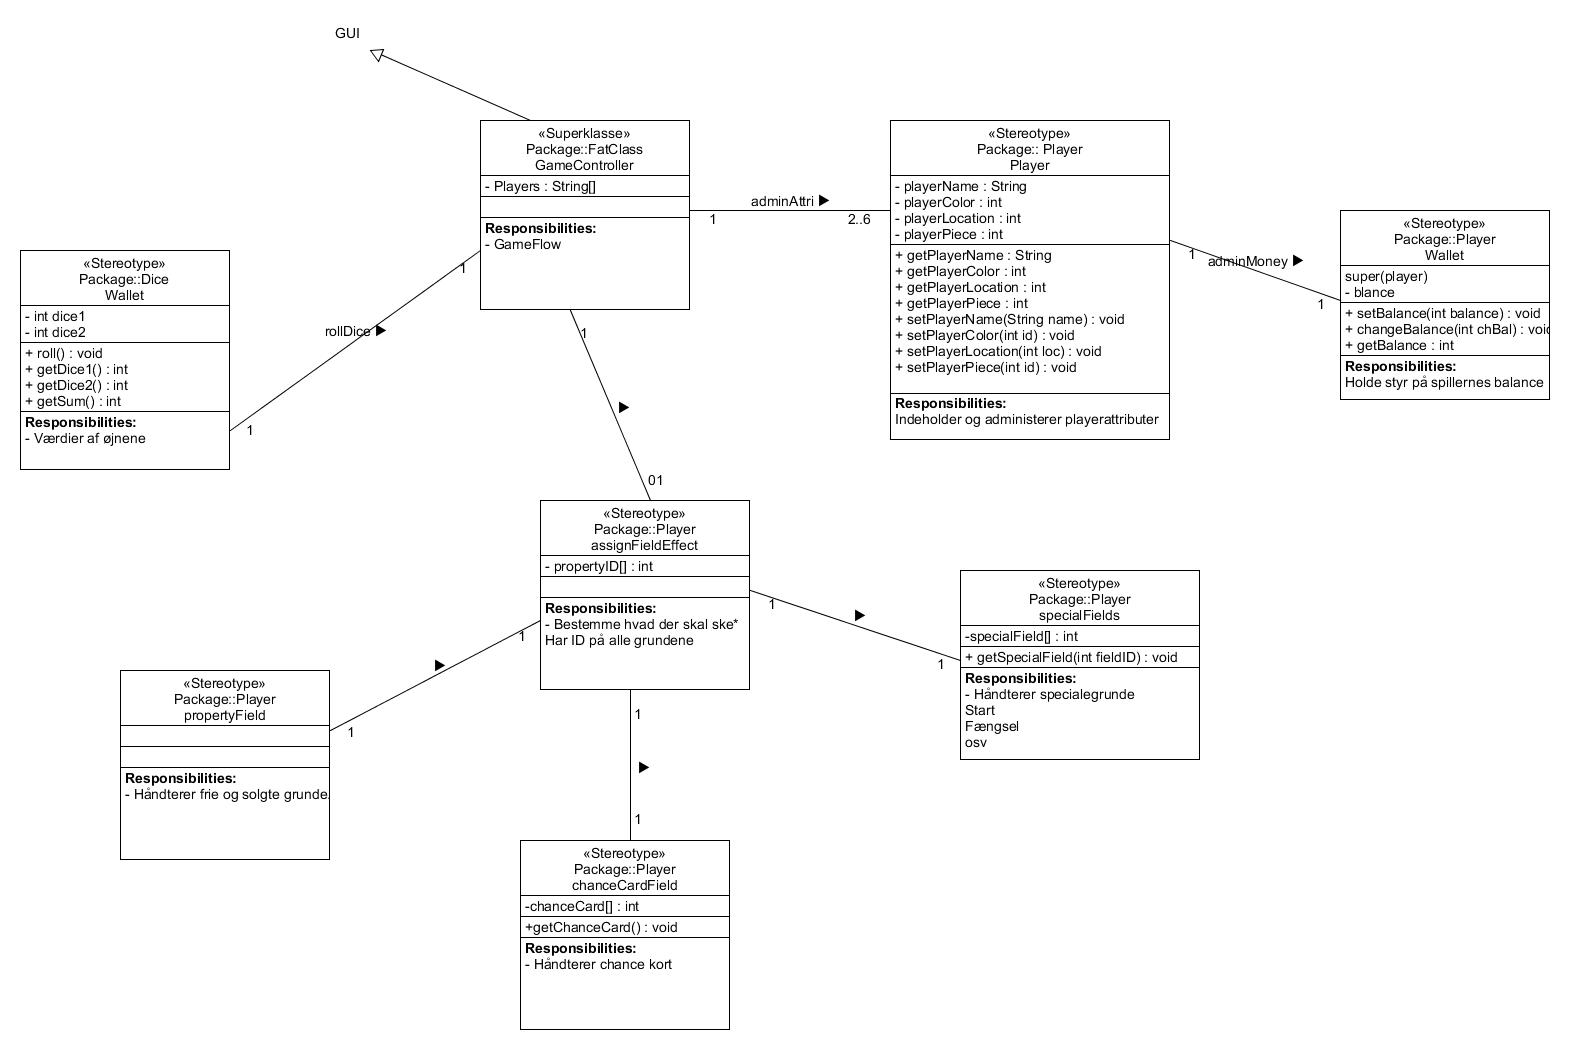
\includegraphics[width=20cm]{fig/Designklassediagram(3).jpg}
            \caption{Klasse diagram tegnet i UMLet}
        \end{figure}
    Klasse diagrammet bygger på vores umiddelbare overvejelser, såvel som vores use case's.
    Dette er for at illusterer sammenspillet mellem vores klasser og deres associationer.
    Dog skal det siges, at dette er en skitse og den aktuelle programmering kan varierer heraf.


\subsection{Sekvensdiagram}
        \begin{figure}[h]
            \advance\leftskip-3cm
            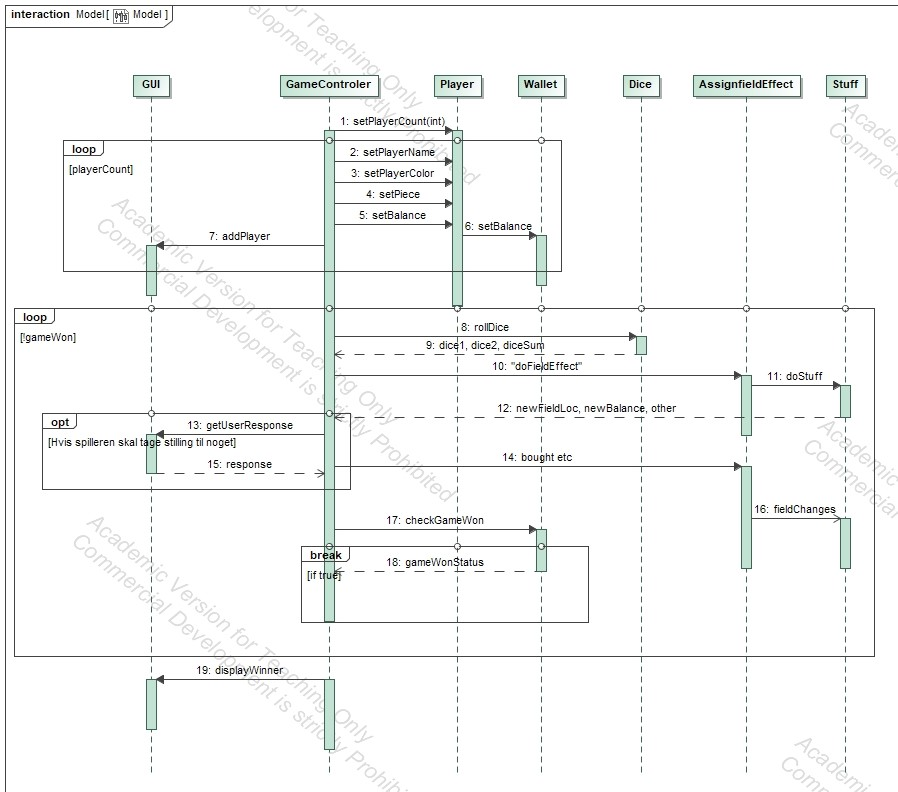
\includegraphics[width=18cm]{fig/Sekvensdiagram(1).jpg}
            \caption{Sekvensdiagram tegnet i MagicDraw}
        \end{figure}
    Vi har her lavet et sekvensdiagram, der skal skabe et overblik over hvordan aktøren, her spilleren,
    kommunikerer med spillet.
\subsection{System sekvensdiagram}
        \begin{figure}[h]
            \advance\leftskip-3cm
            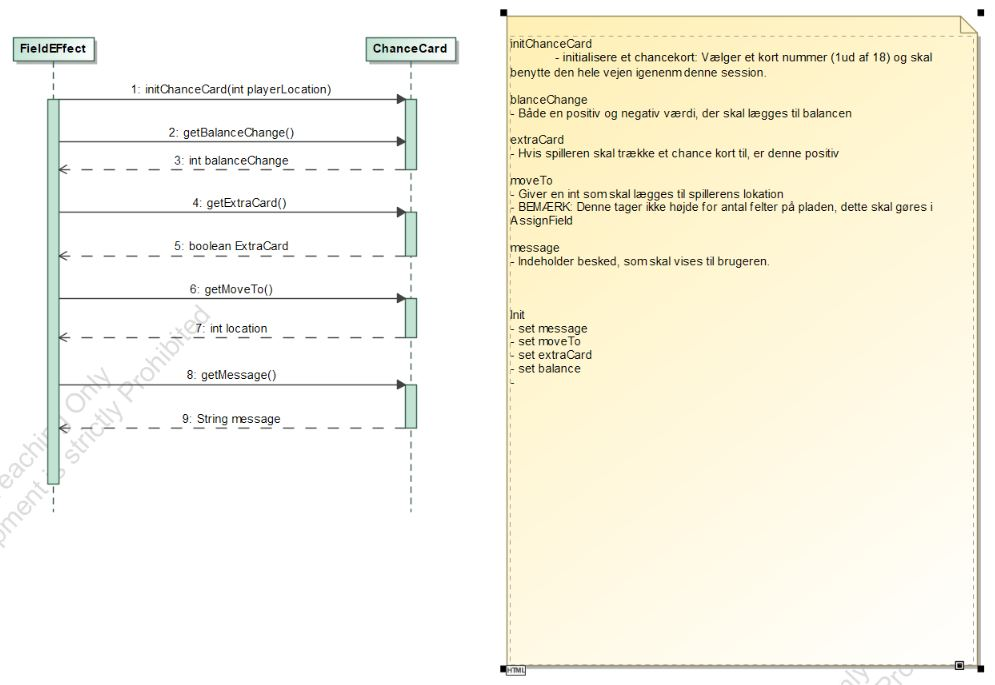
\includegraphics[width=20cm]{fig/SSD.jpg}
            \caption{Systemsekvensdiagram tegnet i MagicDraw}
        \end{figure}
    Vi har her lavet et systemsekvensdiagram for at forhøje gennemsigtigheden ved bruge af
    'chanceCard' klassen.
    %Er dette waste eller ikke, Nicki? :-D
\subsection{Domænemodel}
